\begin{frame}[c]
    \frametitle{多腔红外电光可调谐滤波器:概要}
    \begin{columns}
        \begin{column}{.6\textwidth}
            \begin{itemize}
                \item Gunning, W.; Yeh, P., \textcolor{red}{Multiple-Cavity} \textcolor{pink}{Infrared} \textcolor{purple}{Electro-Optic Tunable} Filter. SPIE: 1980; Vol. 0202.
                \item \textcolor{blue}{重要性:}规避了使用机械调谐结构带来的对温度和颤噪声的敏感。
                \item \textcolor{blue}{瓶颈:}工作波段太窄()。只有不到 $20\ \mathrm{nm}$
                \item \textcolor{blue}{意义:}具有潜在的高传输能力。
                \item \footnotesize{使用的材料:铌酸锂 $\mathrm{LiNbO}_3$,其单晶为光波导,是重要的非线性光学应用材料}
            \end{itemize}
        \end{column}
        \begin{column}{.4\textwidth}
            \begin{figure}[H] %H为当前位置,!htb为忽略美学标准,htbp为浮动图形
                \centering %图片居中
                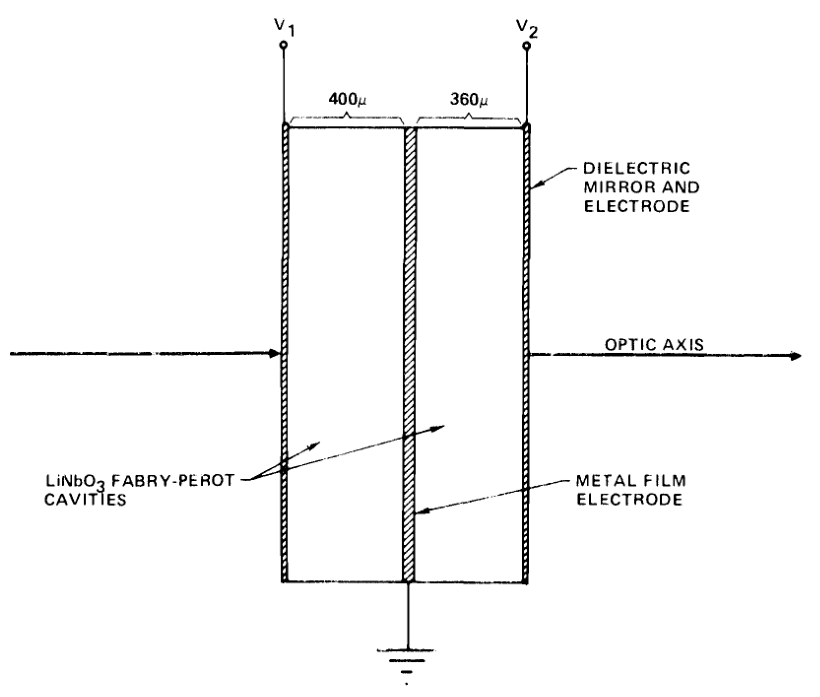
\includegraphics[width=1.\textwidth]{figures/Multiple-Cavity Infrared Electro-Optic Tunable Filter_2.png} %插入图片,[]中设置图片大小,{}中是图片文件名
                \caption{器件结构}
            \end{figure}
        \end{column}
    \end{columns}

    \begin{itemize}
        \item 原理:铌酸锂 $\mathrm{LiNbO}_3$ 是一种特殊的光学材料,在外电场的激励下可产生折射率的改变,由此改变整个谐振腔的共振波长
    \end{itemize}
    器件结构(介质腔相当厚):light $\downarrow$
    \begin{itemize}
        \item Ni 电极 $\rightarrow$ 介质反射镜
        \item $400\ \mathrm{\mu m}\ \mathrm{LiNbO}_3$
        \item $15\ \mathrm{nm}\ \mathrm{Ag}$
        \item $360\ \mathrm{\mu m}\ \mathrm{LiNbO}_3$
        \item 介质反射镜 $\rightarrow$ Ni 电极
    \end{itemize}
\end{frame}

\begin{frame}[c]
    \frametitle{多腔红外电光可调谐滤波器:过程细节}
    \textrm{Ni} 和 \textrm{Ag} 薄膜效果的比较:
    \begin{itemize}
        \item 使用较高 $k/n$ 的值的金属材料效果较好($\mathrm{Ag: }20,\ \mathrm{Ni: }2.3$)
    \end{itemize}

    \begin{figure}[H] %H为当前位置,!htb为忽略美学标准,htbp为浮动图形
        \centering %图片居中
        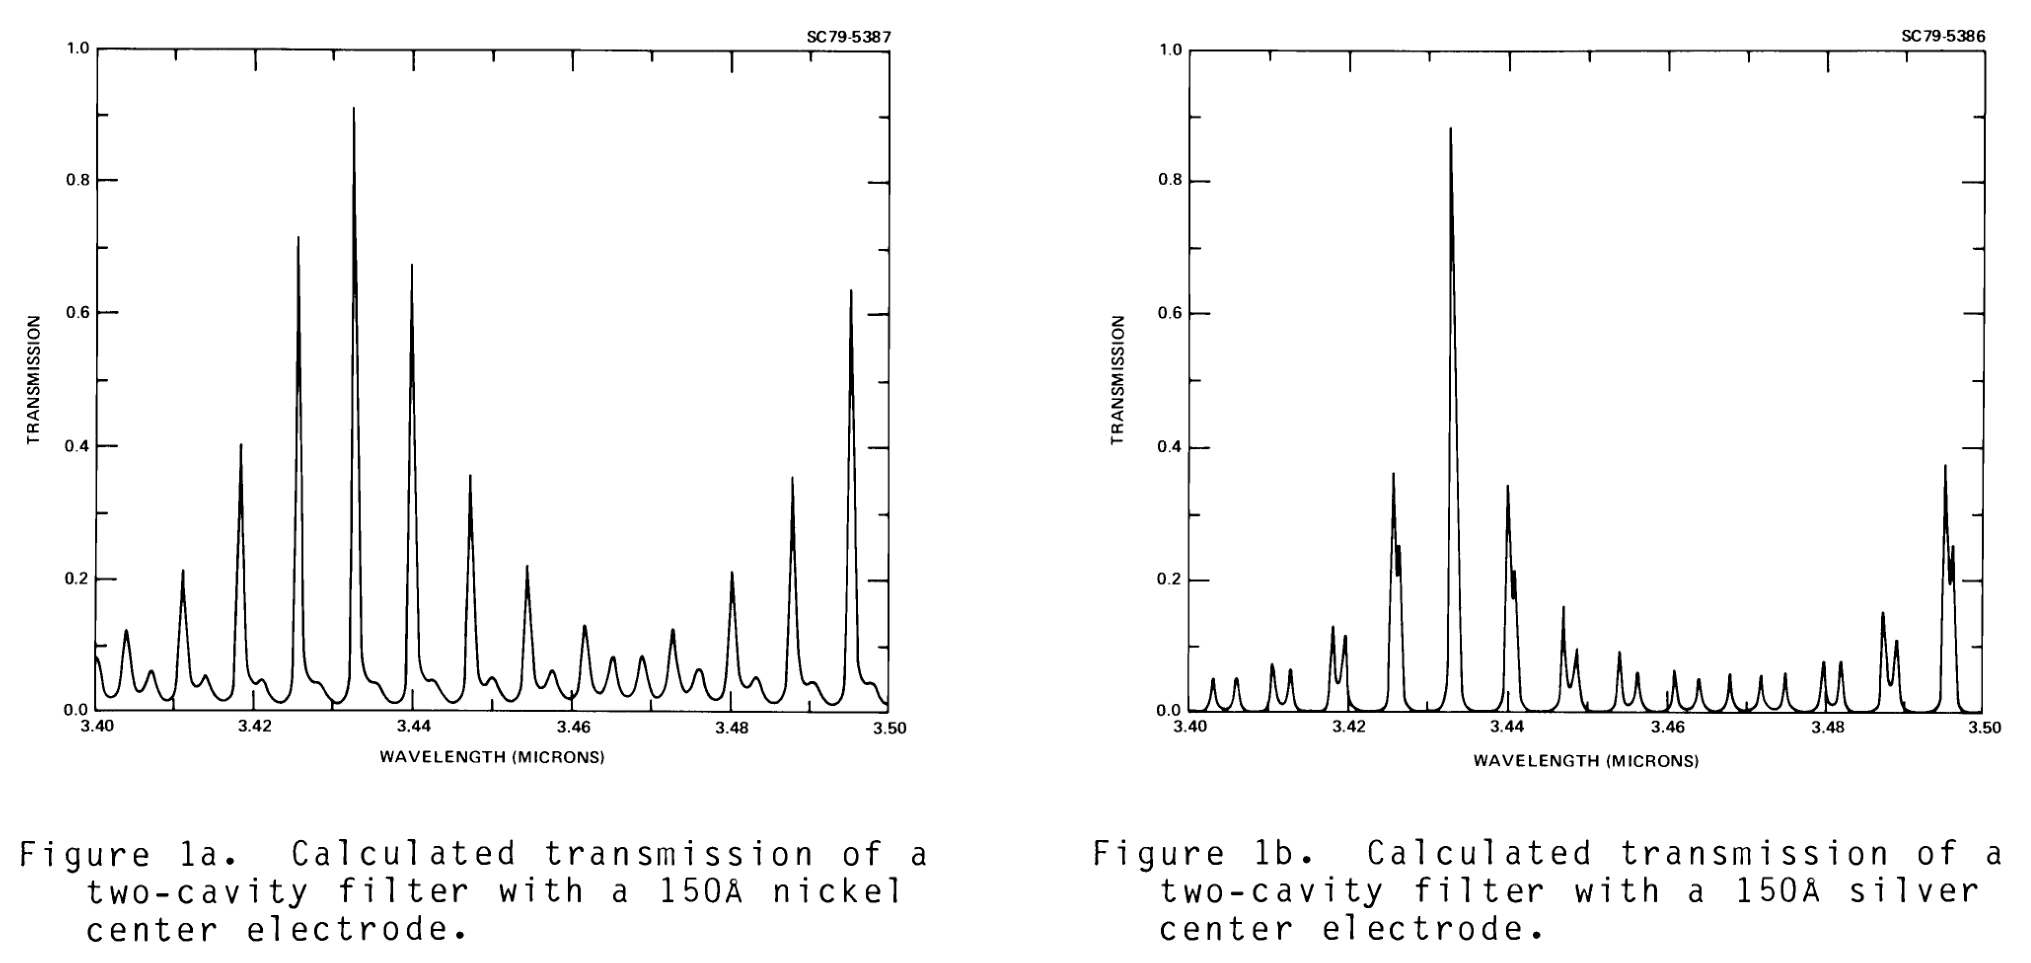
\includegraphics[width=1.\textwidth]{figures/Multiple-Cavity Infrared Electro-Optic Tunable Filter_1.png} %插入图片,[]中设置图片大小,{}中是图片文件名
        \caption{\textrm{Ni} 和 \textrm{Ag} 薄膜的比较}
    \end{figure}
\end{frame}

\begin{frame}[c]
    \frametitle{多腔红外电光可调谐滤波器:仪器性能}
    \begin{itemize}
        \item 可以看到,仪器工作波段只有不到 $20\ \mathrm{nm}$,有待发展。
    \end{itemize}

    \begin{figure}[H] %H为当前位置,!htb为忽略美学标准,htbp为浮动图形
        \centering %图片居中
        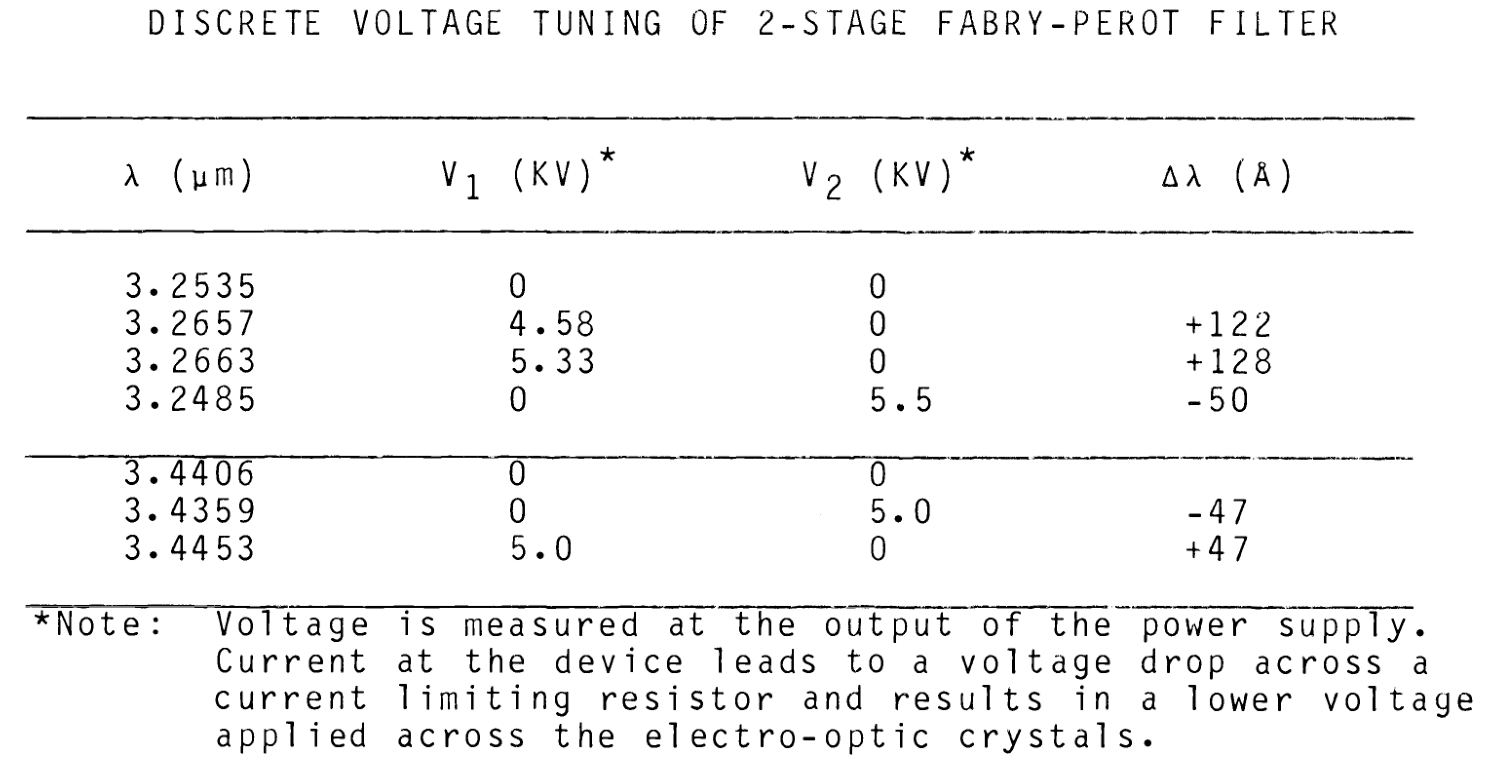
\includegraphics[width=1.\textwidth]{figures/Multiple-Cavity Infrared Electro-Optic Tunable Filter_3.png} %插入图片,[]中设置图片大小,{}中是图片文件名
        \caption{仪器性能}
    \end{figure}
\end{frame}